\chapter{Deployment}
Deploying a unity project for Android and IOS requires the following major deployment tasks that are described below.
\section{Major Deployment Tasks}
	\subsection{Project Setup and Configuration}
	\begin{itemize}
		\item \textbf{Unit Project Setting:}
		\begin{itemize}
			\item {Set up the project in Unity's Build Settings for both iOS and Android.}
			\item {Configure the bundle identifier, version number, orientation, etc.}
			\item {Optimize the Graphics Settings for optimal performance}
		\end{itemize}
		\item \textbf{SDK and Build Tools:}
		\begin{itemize}
			\item {For \textbf{Android}: Install Android \textbf{SDK, NDK,} and \textbf{JDK} via Unity Hub.}
			\item {For \textbf{iOS}: Ensure\textbf{ Xcode} is installed and up to date for building the game.}
		\end{itemize}
	\end{itemize}
	\subsection{Testing and Optimization}
	\begin{itemize}
		\item \textbf{Mobile Specific Testing:}
		\begin{itemize}
			\item {Test the game on a variety of Android and iOS devices}
			\item {Keep an eye on battery life, memory utilization, and frame rates.}
			\item {Examine input handling, touch controls, and UI responsiveness.}
		\end{itemize}
		\item \textbf{Performance Optimization:}
		\begin{itemize}
			\item {Optimize graphics}
			\item {Implement Level of Detail (LOD) for 3D models to enhance performance.}
			\item {Use Profiler and Memory Management tools in Unity to optimize code and improve loading time.}
		\end{itemize}
	\end{itemize}
	\subsection{App Store Compliance}
	\begin{itemize}
		\item \textbf{Android (Google Play):}
		\begin{itemize}
			\item {Prepare the Google Play Console with all required game assets.}
			\item {Ensure APK/Bundle meets Google Play guidelines.}
			\item {Perform testing through Google Play’s pre-launch report for testing.}
		\end{itemize}
		\item \textbf{iOS (Apple App Store):}
		\begin{itemize}
			\item {Upload the iOS build through \textbf{Xcode} or \textbf{Transporter} to \textbf{App Store Connect}.}
			\item {Ensure the app meets Apple’s \textbf{App Store Guidelines}.}
			\item {Prepare \textbf{App Store Connect} with all required assets.}
		\end{itemize}
	\end{itemize}
	\subsection{Distribution of the Product:}
	\begin{itemize}
		\item \textbf{Android (Google Play):}
		\begin{itemize}
			\item {Generate \textbf{APK} or \textbf{AAB} \textbf{(Android App Bundle)} using Unity's build options.}
			\item {Enable \textbf{64-bit support} (required by Google Play).}
			\item {Sign the APK or AAB with your \textbf{release key} for deployment on Google Play.}
			\item {Set up \textbf{beta testing} via the \textbf{Google Play Beta Testing} program for feedback before full release.}
		\end{itemize}
		\item \textbf{iOS (Apple App Store):}
		\begin{itemize}
			\item {Build and export the game to an \textbf{IPA} file through Xcode.}
			\item {Ensure the app is signed with the appropriate \textbf{provisioning profiles} and \textbf{certificates}.}
			\item {Set up \textbf{TestFlight} to beta test the game and gather feedback before public release.}
		\end{itemize}
	\end{itemize}
	\subsection{Analytics, Ads, and Monetization Setup}
	\begin{itemize}
		\item {Integrate\textbf{ Unity Analytics, Google Analytics}, or a third-party service to track user behavior, retention, and engagement.}
		\item {Ensure ads and monetization strategies comply with both Google Play and App Store guidelines.}
	\end{itemize}

\section{Deployment Diagram}

The deployment diagram illustrates the architecture of the Proximity Assault for Android and iOS platforms. The game application includes essential features such as a local inventory system, an in-game AI system, a dummy shop system, and two levels that are stored locally on the device. Future enhancements include the integration of an external server for the shop system to facilitate transactions and Firebase for tracking user data and analytic. Currently, the game does not have cloud-based features or multiplayer support, as depicted in the diagram.\\
\begin{figure}[H]
	\centering
	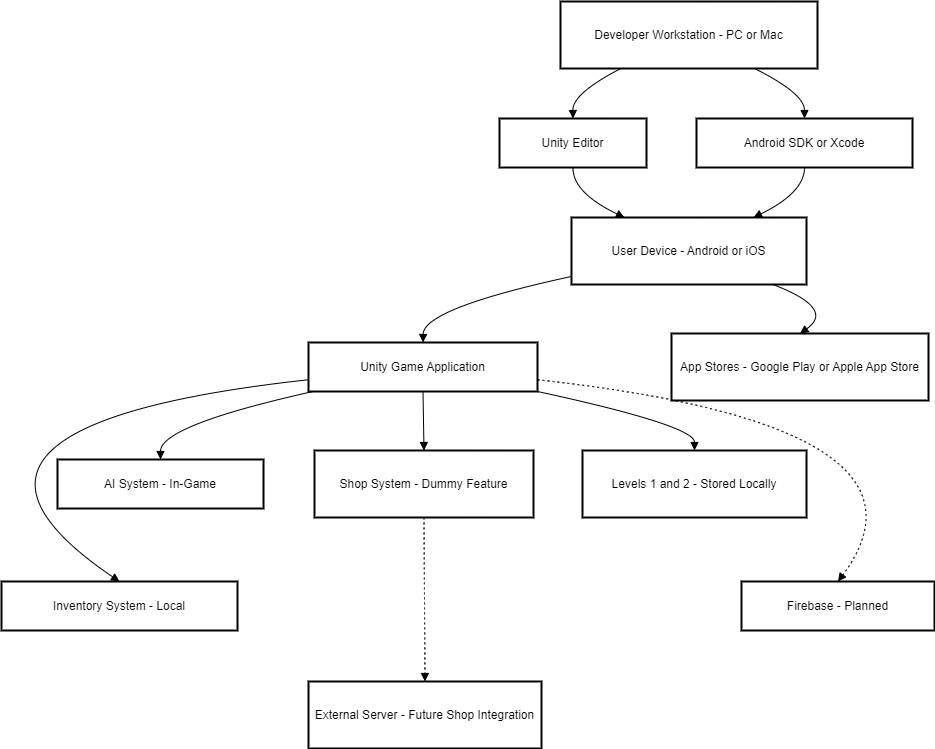
\includegraphics[width=14cm,height=14cm]{C://Users/PMLS/Desktop/Thesis/Latex Thesis/Deployment DiagramM.png}
	\caption{Deployment Diagram}
	\label{fig:Deployement Diagram}
\end{figure}